% \documentclass[handout]{beamer}
\documentclass{beamer}

\mode<presentation>
{
  \usetheme{ANLBlue}
  % \usefonttheme[onlymath]{serif}
  % \usetheme{Singapore}
  % \usetheme{Warsaw}
  % \usetheme{Malmoe}
  % \useinnertheme{circles}
  % \useoutertheme{infolines}
  % \useinnertheme{rounded}

  \setbeamercovered{transparent=5}
}

\usepackage[english]{babel}
\usepackage[latin1]{inputenc}
\usepackage{alltt,listings,multirow,ulem,siunitx}
\usepackage[absolute,overlay]{textpos}
\TPGrid{1}{1}
\usepackage{pdfpages}
\usepackage{ulem}
\usepackage{multimedia}
\usepackage{multicol}
\newcommand\hmmax{0}
\newcommand\bmmax{0}
\usepackage{bm}
\usepackage{comment}
\usepackage{subcaption}

% font definitions, try \usepackage{ae} instead of the following
% three lines if you don't like this look
\usepackage{mathptmx}
\usepackage[scaled=.90]{helvet}
% \usepackage{courier}
\usepackage[T1]{fontenc}
\usepackage{tikz}
\usetikzlibrary{decorations.pathreplacing}
\usetikzlibrary{shadows,arrows,shapes.misc,shapes.arrows,shapes.multipart,arrows,decorations.pathmorphing,backgrounds,positioning,fit,petri,calc,shadows,chains,matrix,mindmap}

\newcommand\vvec{\bm v}
\newcommand\bvec{\bm b}
\newcommand\bxk{\bvec_0 \times \kappa_0 \cdot \nabla}
\newcommand\delp{\nabla_\perp}

% \usepackage{pgfpages}
% \pgfpagesuselayout{4 on 1}[a4paper,landscape,border shrink=5mm]

\usepackage{JedMacros}

\newcommand{\timeR}{t_{\mathrm{R}}}
\newcommand{\timeW}{t_{\mathrm{W}}}
\newcommand{\mglevel}{\ensuremath{\ell}}
\newcommand{\mglevelcp}{\ensuremath{\mglevel_{\mathrm{cp}}}}
\newcommand{\mglevelcoarse}{\ensuremath{\mglevel_{\mathrm{coarse}}}}
\newcommand{\mglevelfine}{\ensuremath{\mglevel_{\mathrm{fine}}}}

%solution and residual
\newcommand{\vx}{\ensuremath{x}}
\newcommand{\vc}{\ensuremath{\hat{x}}}
\newcommand{\vr}{\ensuremath{r}}
\newcommand{\vb}{\ensuremath{b}}

%operators
\newcommand{\vA}{\ensuremath{A}}
\newcommand{\vP}{\ensuremath{I_H^h}}
\newcommand{\vS}{\ensuremath{S}}
\newcommand{\vR}{\ensuremath{I_h^H}}
\newcommand{\vI}{\ensuremath{\hat I_h^H}}
\newcommand{\vV}{\ensuremath{\mathbf{V}}}
\newcommand{\vF}{\ensuremath{F}}
\newcommand{\vtau}{\ensuremath{\mathbf{\tau}}}


\title{HPGMG: Relevant Benchmarking for Scientific Computing}
\subtitle{This talk: \url{http://59A2.org/files/20150525-HPGMG.pdf}}

\author{{\bf Jed Brown} \texttt{jed@jedbrown.org} (ANL and CU Boulder)\\
{\small HPGMG Collaborators: Mark Adams, Sam Williams, John Shalf, Erich Strohmeier (LBNL)}}

% - Use the \inst command only if there are several affiliations.
% - Keep it simple, no one is interested in your street address.
% \institute
% {
%   Mathematics and Computer Science Division \\ Argonne National Laboratory
% }

\date{HPCSE, Czech Republic, 2015-05-25}

% This is only inserted into the PDF information catalog. Can be left
% out.
\subject{Talks}


% If you have a file called "university-logo-filename.xxx", where xxx
% is a graphic format that can be processed by latex or pdflatex,
% resp., then you can add a logo as follows:

% \pgfdeclareimage[height=0.5cm]{university-logo}{university-logo-filename}
% \logo{\pgfuseimage{university-logo}}



% Delete this, if you do not want the table of contents to pop up at
% the beginning of each subsection:
% \AtBeginSubsection[]
% {
% \begin{frame}<beamer>
%   \frametitle{Outline}
%   \tableofcontents[currentsection,currentsubsection]
% \end{frame}
% }

\AtBeginSection[]
{
  \begin{frame}<beamer>
    \frametitle{Outline}
    \tableofcontents[currentsection]
  \end{frame}
}

% If you wish to uncover everything in a step-wise fashion, uncomment
% the following command:

% \beamerdefaultoverlayspecification{<+->}

\begin{document}
\lstset{language=C}
\normalem

\begin{frame}
  \titlepage
\end{frame}

\begin{frame}{What is performance?}
  \begin{block}{Dimensions}
    \begin{itemize}
    \item Model complexity
    \item Accuracy
    \item Time
      \begin{itemize}
      \item per problem instance
      \item for the first instance
      \item compute time versus human time
      \end{itemize}
    \item Cost
      \begin{itemize}
      \item incremental cost
      \item subsidized?
      \end{itemize}
    \end{itemize}
  \end{block}
  \begin{itemize}
  \item Terms relevant to scientist/engineer
  \item Compute meaningful quantities -- needed to make a decision or obtain a result of scientific value---not one iteration/time step
  \item No flop/s, number of elements/time steps
  \end{itemize}
\end{frame}

\begin{frame}{Work-precision diagram: \emph{de rigueur} in ODE community}
  \begin{center}
    \includegraphics[width=0.8\textwidth]{figures/HairerWanner-WorkPrecision.png}\\
    {\scriptsize [Hairer and Wanner (1999)]}
  \end{center}
  \begin{itemize}
  \item Tests discretization, adaptivity, algebraic solvers, implementation
  \item No reference to number of time steps, flop/s, etc.
  \item Useful performance results inform \emph{decisions} about \emph{tradeoffs}.
  \end{itemize}
\end{frame}

\begin{frame}{Strong Scaling: cost-time tradeoff}
  \begin{center}
    \includegraphics[width=.75\textwidth]{figures/olenz/olenz-time-np}
  \end{center}
  \vspace{-1em}
  \begin{itemize}
  \item Good: shows absolute time
  \item Bad: log-log plot makes it difficult to discern efficiency
    \begin{itemize}
    \item Stunt 3: \url{http://blogs.fau.de/hager/archives/5835}
    \end{itemize}
  \item Bad: plot depends on problem size
  \end{itemize}
\end{frame}

\begin{frame}{Strong Scaling: cost-time tradeoff}
  \begin{center}
    \includegraphics[width=.75\textwidth]{figures/olenz/olenz-efficiency-np}
  \end{center}
  \begin{itemize}
  \item Good: shows efficiency at scale
  \item Bad: no absolute time, depends on problem size
  \end{itemize}
\end{frame}

\begin{frame}{Strong Scaling: cost-time tradeoff}
  \begin{center}
    \includegraphics[width=.75\textwidth]{figures/olenz/olenz-efficiency-time}
  \end{center}
  \begin{itemize}
  \item Good: absolute time, absolute efficiency (like DOF/s/cost)
  \item Good: independent of problem size for perfect weak scaling
  \item Bad: hard to see machine size (but less important)
  \end{itemize}
\end{frame}

\begin{frame}{Exascale Science \& Engineering Demands}
  \begin{itemize}
  \item Model fidelity: resolution, multi-scale, coupling
    \begin{itemize}
    \item Transient simulation is not weak scaling: $\Delta t \sim \Delta x$
    \end{itemize}
  \item Analysis using a sequence of forward simulations
    \begin{itemize}
    \item Inversion, data assimilation, optimization
    \item Quantify uncertainty, risk-aware decisions
    \end{itemize}
  \item Increasing relevance $\implies$ external requirements on time
    \begin{itemize}
    \item Policy: 5 SYPD to inform IPCC
    \item Weather, manufacturing, field studies, disaster response
    \end{itemize}
  \item ``weak scaling'' [\ldots] will increasingly give way to ``strong scaling''\\
    {\scriptsize [The International Exascale Software Project Roadmap, 2011]}
  \item ACME @ \SI{25}{\kilo\metre} scaling saturates at $<10\%$ of Titan (CPU) or Mira
    \begin{itemize}
    \item Cannot decrease $\Delta x$: SYPD would be too slow to calibrate
    \item ``results'' would be meaningless for 50-100y predictions, a ``stunt run''
    \end{itemize}
  \item \alert{\bf ACME v1 goal of 5 SYPD is pure strong scaling.}
    \begin{itemize}
    \item Likely faster on Edison (2013) than any DOE machine --2020
    \item Many non-climate applications in same position.
    \end{itemize}
  \end{itemize}
\end{frame}

\begin{frame}{HPL and the Top500 list}
  \begin{center}
    \includegraphics[width=0.9\textwidth]{figures/Supercomputers-history.pdf}
  \end{center}
  \begin{itemize}
  \item High Performance LINPACK
  \item Solve $n\times n$ dense linear system: $\bigO(N^{3/2})$ flops on $N=n^2$ data
  \item Top500 list created in 1993 by Hans Meuer, Jack Dongarra, Erich
    Strohmeier, Horst Simon
  \end{itemize}
\end{frame}

\begin{frame}{Role of HPL}
  \begin{itemize}
  \item The major centers have their own benchmark suites (e.g., CORAL)
  \item Nobody (vendors or centers) will say they built an HPL machine
  \item HPL ranking and peak flop/s are still used for press releases
  \item Machines need to be justified to politicians holding the money
    \begin{itemize}
    \item Politicians are vulnerable to propaganda and claims of inefficient spending
    \end{itemize}
  \item It is naive to believe HPL has no influence on procurement or on scientists' expectations
  \end{itemize}
\end{frame}

\begin{frame}
  \includegraphics[width=\textwidth]{figures/karlrupp/flop-per-byte-dp.pdf} \\
  {\scriptsize [c/o Karl Rupp]}
\end{frame}

\begin{frame}{It's all about the memory}
  \begin{center}
    \includegraphics[width=.65\textwidth]{figures/Ang-CPUGPU.png}
    \includegraphics[width=.35\textwidth]{figures/Ang-AMDLlano.png} \\
    {\scriptsize [Ang et al, 2014]}
  \end{center}
  \begin{itemize}
  \item Memory motion dominates floating point cost
  \item About half of die devoted to caches
  \item Network moving on-die, maybe throughput cores
  \item High-bandwidth on-package memory may have \emph{worse} latency than DRAM
  \end{itemize}
\end{frame}

\begin{frame}{Arithmetic intensity is not enough}
  \begin{center}
    \includegraphics[width=\textwidth]{figures/hardware/MKL-dgeqrf-20150525.png} \\
    \includegraphics[width=\textwidth]{figures/hardware/MKL-dgetrf-20150525.png}
  \end{center}
  \begin{itemize}
  \item QR and LU factorization have same complexity.
  \item Stable QR factorization involves more synchronization.
  \item Synchronization is much more expensive on Xeon Phi.
  \end{itemize}
\end{frame}

\begin{frame}{Algorithms keep pace with hardware (sometimes)}
  \includegraphics[width=\textwidth]{figures/KeyesAlgorithmsKeepPace.png} \\
  {\scriptsize [c/o David Keyes]}
  \begin{itemize}
  \item Opportunities now: uncertainty quantification, design
  \item Incentive to find optimal algorithms for more applications
  \end{itemize}
\end{frame}

\begin{frame}{What does ``representative'' mean?}
  \begin{itemize}
  \item Diverse applications
    \begin{itemize}
    \item Explicit PDE solvers (seismic wave propagation, turbulence)
    \item Implicit PDE solvers and multigrid methods (geodynamics, structural mechanics, steady-state RANS)
    \item Irregular graph algorithms (network analysis, genomics, game trees) 
    \item Dense linear algebra and tensors (quantum chemistry) 
    \item Fast methods for N-body problems (molecular dynamics, cosmology) 
    \item Cross-cutting: data assimilation, uncertainty quantification
    \end{itemize}
  \item Diverse external requirements
    \begin{itemize}
    \item Real-time, policy, manufacturing
    \item Privacy
    \item In-situ processing of experimental data
    \item Mobile/energy limitations
    \end{itemize}
  \end{itemize}
\end{frame}

\begin{frame}{Necessary and sufficient}
  \begin{block}{Goodhart's Law}
    When a measure becomes a target, it ceases to be a good measure.
  \end{block}

  \begin{itemize}
  \item Features stressed by benchmark \textbf{necessary} for some apps
  \item Performance on benchmark \textbf{sufficient} for most apps
  \end{itemize}
\end{frame}

\begin{frame}{HPGMG: a new benchmarking proposal}
  \begin{itemize}
  \item \url{https://hpgmg.org}, hpgmg-forum@hpgmg.org mailing list
  \item Mark Adams, Sam Williams (finite-volume), Jed (finite-element), John Shalf, Brian Van Straalen, Erich Strohmeier, Rich Vuduc
  \item Gathering momentum, SC14 BoF
  \item Implementations
    \begin{description}
    \item[Finite Volume] memory bandwidth intensive, simple data dependencies, 2nd and 4th order
    \item[Finite Element] compute- and cache-intensive, vectorizes, overlapping writes
    \end{description}
  \item Full multigrid, well-defined, scale-free problem
  \item Matrix-free operators, Chebyshev smoothers
  \end{itemize}
\end{frame}

\begin{frame}[fragile]
  \frametitle{Full Multigrid (FMG): Prototypical Fast Algorithm}
  \begin{figure}
  \centering
  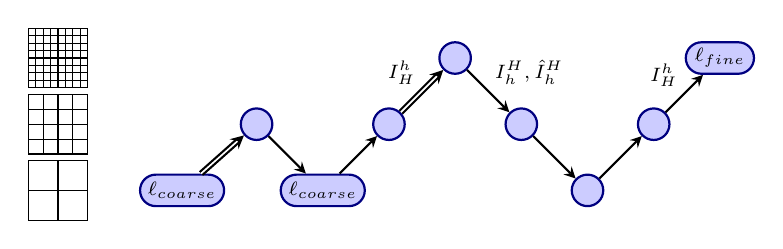
\begin{tikzpicture}
    [>=stealth,
    every node/.style={inner sep=2pt},
    restrict/.style={thick},
    prolong/.style={thick},
    mglevel/.style={rounded rectangle,draw=blue!50!black,fill=blue!20,thick,minimum size=4mm},
    ]
    \begin{scope}\scriptsize
      \newcommand\mgdx{3.0em}
      \newcommand\mgdy{3.0em}
      \newcommand\mgl[1]{(pow(2,#1+1))}
      \newcommand\mgloc[4]{(#1 + #4*\mgdx*#3,#2 + \mgdy*#3)}

      \node[mglevel] (coarseinit) at \mgloc{-3}{0}{0}{0} {$\mglevel_{coarse}$};

      \node[mglevel] (afine) at \mgloc{0}{0}{1}{1} {};

      \node[mglevel] (bcoarse) at \mgloc{2*\mgdx}{0}{0}{1} {$\mglevel_{coarse}$};
      \node[mglevel] (bup1) at \mgloc{2*\mgdx}{0}{1}{1} {};
      \node[mglevel] (bfine) at \mgloc{2*\mgdx}{0}{2}{1} {};

      \node[mglevel] (cdown1) at \mgloc{6*\mgdx}{0}{1}{-1} {};
      \node[mglevel] (ccoarse) at \mgloc{6*\mgdx}{0}{0}{-1} {};
      \node[mglevel] (cup1) at \mgloc{6*\mgdx}{0}{1}{1} {};
      \node[mglevel] (cfine) at \mgloc{6*\mgdx}{0}{2}{1} {$\mglevel_{fine}$};


      \draw[->,restrict,double]
                         (coarseinit) -- node [above right] {} (afine);
      \draw[->,restrict]
                         (afine) -- node [above right] {} (bcoarse);
      \draw[->,restrict]
                         (bcoarse) -- node [above right] {} (bup1);
      \draw[->,restrict,double]
                         (bup1) -- node [above left] {$\mathbb I_H^h$} (bfine);
      \draw[->,restrict]
                         (bfine) -- node [above right] {$I_h^H,\hat I_h^H$} (cdown1);
      \draw[->,restrict]
                         (cdown1) -- node [above right] {} (ccoarse);
      \draw[->,restrict]
                         (ccoarse) -- node [above right] {} (cup1);
      \draw[->,restrict]
                         (cup1) -- node [above left] {$I_H^h$} (cfine);

      %grids
      \newcommand\mghx{0.9*\mgdx}
      \newcommand\mghy{0.9*\mgdy}

      \draw[shift=\mgloc{-2*\mgdx}{0}{2}{0},
      xstep=\mghy/\mgl{2},
      ystep=\mghy/\mgl{2}]
      (-0.5*\mghy,-0.5*\mghy) grid (0.5*\mghy,0.5*\mghy);

      \draw[shift=\mgloc{-2*\mgdx}{0}{1}{0},
      xstep=\mghy/\mgl{1},
      ystep=\mghy/\mgl{1}]
      (-0.5*\mghy,-0.5*\mghy) grid (0.5*\mghy,0.5*\mghy);

      \draw[shift=\mgloc{-2*\mgdx}{0}{0}{0},
      xstep=\mghy/\mgl{0},
      ystep=\mghy/\mgl{0}]
      (-0.5*\mghy,-0.5*\mghy) grid (0.5*\mghy,0.5*\mghy);

  \end{scope}
\end{tikzpicture}
\label{fig:FMG}
\end{figure}
\begin{itemize}
  \item start with coarse grid
  \item truncation error within one cycle
  \item about five work units for many problems
  \item no ``fat'' left to trim -- robust to gaming
  \item distributed memory -- restrict active process set using Z-order
    \begin{itemize}
    \item $\bigO(\log^2 N)$ parallel complexity stresses network
    \end{itemize}
  \item scale-free specification
    \begin{itemize}
    \item no mathematical reward for decomposition granularity
    \item don't have to adjudicate ``subdomain''
    \end{itemize}
\end{itemize}
\end{frame}

\begin{frame}{Multigrid design decisions}
  \begin{itemize}
  \item $Q_2$ finite elements
    \begin{itemize}
    \item Partition of work not partition of data -- sharing/overlapping writes
    \item $Q_2$ is a middle-ground between lowest order and high order
    \item Matrix-free pays off, tensor-product element evaluation
    \end{itemize}
  \item Linear elliptic equation with manufactured solution
  \item Mapped coordinates
    \begin{itemize}
    \item More memory streams, increase working set, longer critical path
    \end{itemize}
  \item No reductions
    \begin{itemize}
    \item Coarse grid is strictly more difficult than reduction
    \item Not needed because FMG is a direct method
    \end{itemize}
  \item Chebyshev/Jacobi smoothers, $V(3,1)$ cycle
    \begin{itemize}
    \item Multiplicative smoothers hard to verify in parallel
    \item Avoid intermediate scales (like Block Jacobi/Gauss-Seidel)
    \end{itemize}
  \item Full Approximation Scheme
  \end{itemize}
\end{frame}

% \begin{frame}{How much parallelism out of how much cache?}
%   \begin{tabular}{l rrrr rr}
%     \toprule
%     Processor & v width & threads & F/inst & latency & L1D & L1D/\#par \\
%     \midrule
%     Nehalem & 2 & 1 & 2 & 5 & 32 KiB & 1638 B \\
%     Sandy Bridge & 4 & 2 & 2 & 5 & 32 KiB & 819 B \\
%     Haswell & 4 & 2 & 4 & 5 & 32 KiB & 410 B \\
%     BG/P & 2 & 1 & 2 & 6 & 32 KiB & 1365 B \\
%     BG/Q & 4 & 4 & 2 & 6 & 32 KiB & 682 B \\
%     KNC & 8 & 4 & 4 & 5 & 32 KiB & 205 B \\
%     Tesla K20 & 32 & * & 2 & 10 & 64 KiB & 102 B \\
%     \bottomrule
%   \end{tabular}
%   \begin{itemize}
%   \item Most ``fast'' algorithms do about $O(N)$ flops on $N$ data
%   \item xGEMM does $O(N^{3/2})$ flops on $N$ data
%   \item Exploitable parallelism limited by cache and register load/store
%   \item L2/L3 performance highly variable between architectures
%   \end{itemize}
% \end{frame}

\begin{frame}{SuperMUC (FDR 10, E5-2680)}
  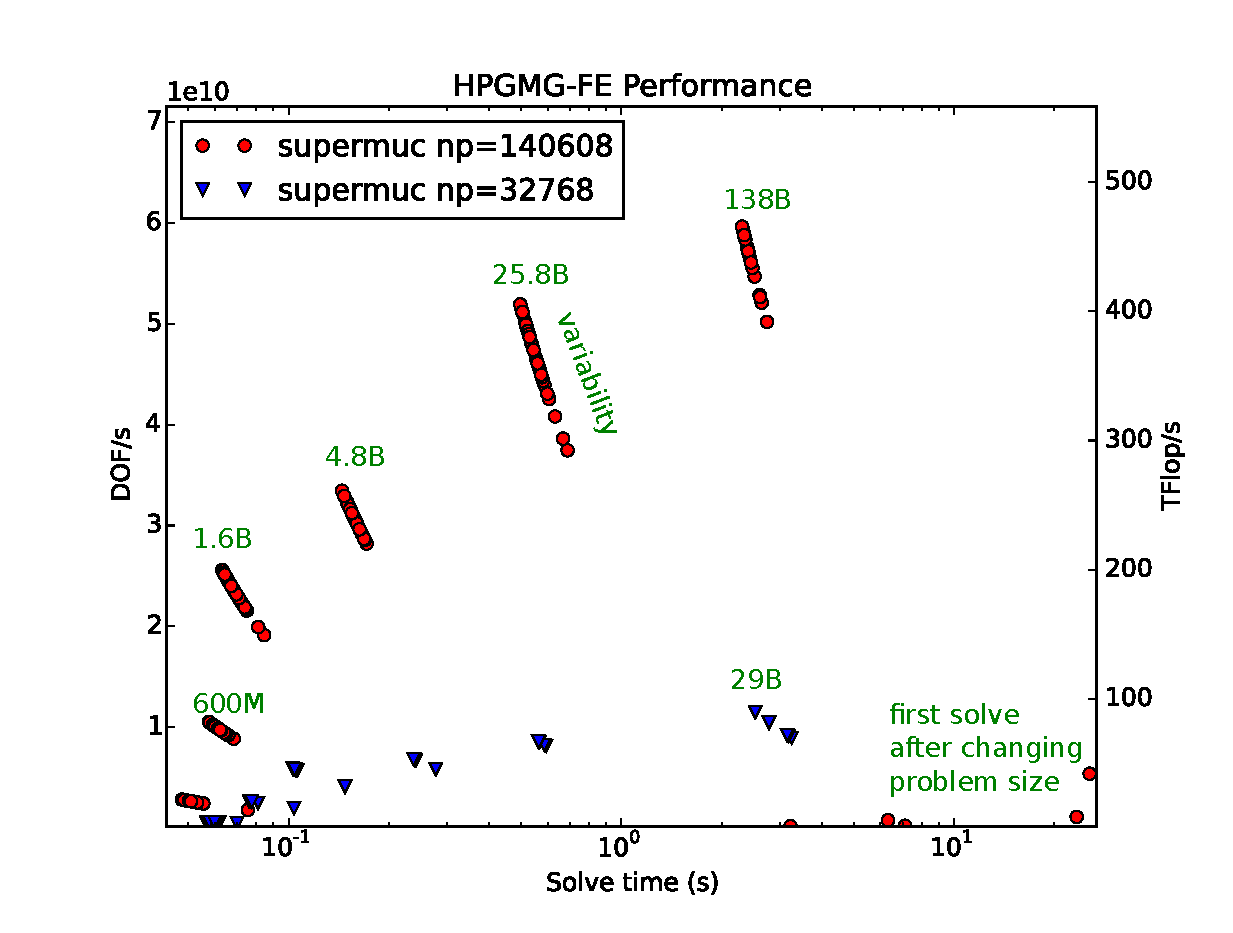
\includegraphics[width=\textwidth]{figures/hpgmg/range-supermuc-ann.eps}
\end{frame}

\begin{frame}{Edison (Aries, E5-2695v2)}
  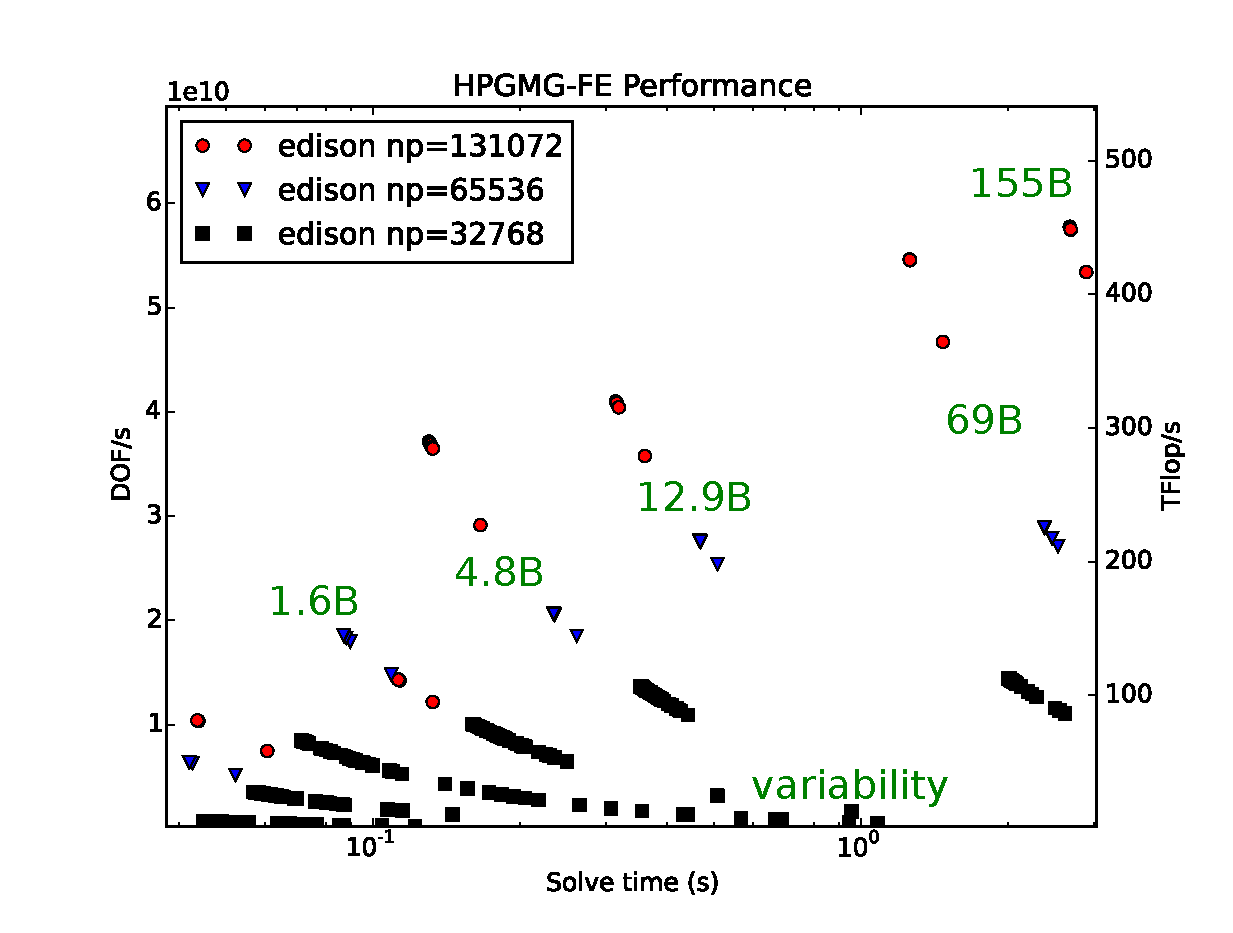
\includegraphics[width=\textwidth]{figures/hpgmg/range-edison-ann.eps}
\end{frame}

\begin{frame}{HPGMG-FE on Edison, SuperMUC, Titan}
  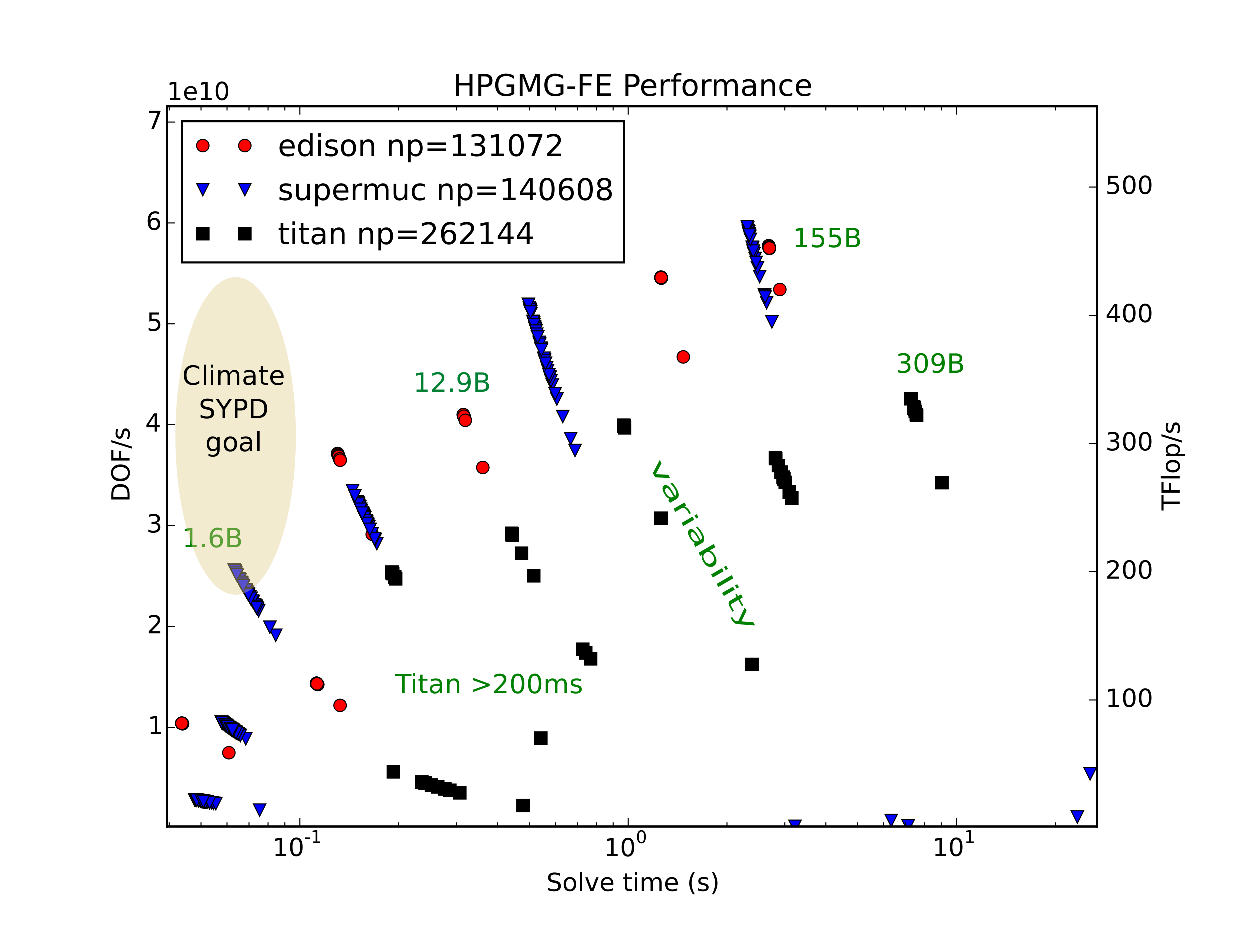
\includegraphics[width=\textwidth]{figures/hpgmg/range-edison-supermuc-titan-ann2.eps}
\end{frame}

\begin{frame}{Kiviat diagrams}
  \begin{center}
    \includegraphics[width=\textwidth]{figures/hpgmg-kiviat-20140606.png}
  \end{center}
  \begin{itemize}
  \item c/o Ian Karlin and Bert Still (LLNL)
  \end{itemize}
\end{frame}

\begin{frame}{HPGMG-FV distinguishes networks at 2M DOFs/node}
  \begin{center}
    \includegraphics[width=\textwidth]{figures/hpgmg/hpgmg-fv-201408-flatmpi-vs-openmp.pdf}
  \end{center}
\end{frame}

\begin{frame}{MIC communication bottlenecks on Stampede}
  \begin{center}
    \includegraphics[width=\textwidth]{figures/hpgmg/fv-mic-mpi.png}
  \end{center}
\end{frame}

\begin{frame}{Outlook}
  \begin{itemize}
  \item What is the cost of performance variability?
    \begin{itemize}
    \item Measure best performance, average, median, 10th percentile?
    \item Applications bundling due to perverse queue incentives
    \end{itemize}
  \item Should dynamic range enter into a ranking metric?
    \begin{itemize}
    \item Why is NERSC installing DRAM in Cori?
    \item Versatility is an essential part of Performance.
    \end{itemize}
  \item Finite element or finite volume?
    \begin{itemize}
    \item overlapping writes, cache reuse
    \item FE: $>20\%$ Intel, $6\%$ Blue Gene/Q; vs $10\%$ for FV
    \item FV: 4th order (higher AI) improves flop/s on Intel, not on BG/Q
    \item FV 4th order performs best with ``red-black GS'' -- weak order dependence
    \end{itemize}
  \item Linear or nonlinear?
  \item Irregularity and adaptivity?
  \item Tensor-valued coefficients?
  \item Elasticity?
  \item HPGMG does not seek to address I/O.
  \end{itemize}
\end{frame}

\end{document}
